\documentclass[a4paper,12p]{article}
\usepackage{standalone}
\usepackage{polski}
\usepackage[utf8]{inputenc}
\usepackage{amsmath}
\usepackage{physics}
\usepackage{amsfonts}
\usepackage{mathtools}
\usepackage{algorithm}% http://ctan.org/pkg/algorithms
\usepackage{algpseudocode}% http://ctan.org/pkg/algorithmicx
\usepackage{tikz}
\usepackage{amssymb}
\usepackage{indentfirst}
\linespread{1.5}

\renewcommand{\refname}{Źródła}
\newcommand\tab[1][1cm]{\hspace*{#1}}

\begin{document}

\begin{titlepage}
	\begin{center}
	
	{\huge\bfseries Algorytmy zaawansowane - projekt\par}
	\vspace{1cm}
	{\Large\scshape Wiktor Gontarczyk\par}
	{\Large\scshape Tomasz Laskowski\par}
	\vspace{2cm}

	\today
	\vspace{1cm}	
	
	\end{center}
\end{titlepage}

\tableofcontents

\newpage

\section{Cel projektu}

Celem projektu jest zaproponowanie algorytmu pozwalającego na wygenerowanie drzewa na podstawie macierz odległości pomiędzy wierzchołkami.


\section{Przedstawienie problemu}

Rozpatrzmy kwadratową, symetryczną macierz $D=[d_{ij}]_{n \times n}$ o wyrazach naturalnych. 

Problem $P$ o rozmiarze $n$ dla macierzy $D$ definiujemy jako zadania znalezienia (zbudowania) grafu nieskierowanego $G$ o zbiorze wierzchołków $V = v_1, v_2, \cdots v_n $ i zbiorze krawędzi $E \in (V \times V)^n$, t. że graf $G$ jest drzewem oraz dla każdej pary wierzchołków $v_i, v_j \in V$, długość ścieżki pomiędzy nimi wynosi $d_{ij}$.

\section{Kod Prüfera}

Dla $n \in \mathbb{N}, n > 3$, kod Prüfera jest ciągiem $n - 2$ liczb od $1$ do $n$.

Kodowaniem Prüfera będziemy nazywać algorytm przyjmujący na wejściu drzewo $T$ o $n$ wierzchołkach i zwracający odpowiadający mu kod Prüfera. Zakładamy, że wierzchołki posiadają etykiety od $1$ do $n$.

\begin{algorithm}
		\floatname{algorithm}{Algorytm}
		\caption{Kodowanie Prüfera}
		\label{algo}
		$P$ = $\{ \}$ \\
		powtórz $n-2$ razy: \\
			\tab $v =$ liść o najniższej etykiecie w $T$ \\
			\tab dodaj do $P$ etykietę sąsiada $v$ \\
			\tab usuń $v$ z $T$ \\
		zwróć $P$
\end{algorithm}

Przykład dla $P = ( 3, 3, 4, 4 )$:

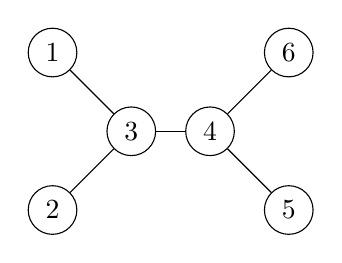
\begin{tikzpicture}
	\node[shape=circle,draw=black] (1) at (0,2) {1};
	\node[shape=circle,draw=black] (2) at (0,0) {2};
	\node[shape=circle,draw=black] (3) at (1,1) {3};
	\node[shape=circle,draw=black] (4) at (2,1) {4};
	\node[shape=circle,draw=black] (5) at (3,0) {5};
	\node[shape=circle,draw=black] (6) at (3,2) {6};
	
	\path [-] (1) edge node[left] {} (3);
	\path [-] (2) edge node[left] {} (3);
	\path [-] (3) edge node[left] {} (4);
	\path [-] (4) edge node[left] {} (5);
	\path [-] (4) edge node[left] {} (6);
\end{tikzpicture}

Dekodowaniem Prüfera nazywamy odwrotną operację tzn. otrzymanie kodu Prüfera odpowiadającego wejsciowemu drzewu $T$ o etykietowanych wierzchołkach. Przez $p_i$ będziemy oznaczać $i$-ty element kodu Prüfera $P$.

\begin{algorithm}
		\floatname{algorithm}{Algorytm}
		\caption{Dekodowanie Prüfera}
		\label{algo}
		
		$n = |P| + 2$ \\
		$V = \{ 1, 2, \cdots n \}$ \\
		$T = $ graf o $n$ wierzchołkach bez krawędzi \\
		dla $i$ od $1$ do $n-2$: \\
			\tab $v =$ wierzchołek o etykiecie będącej najmniejszą wartością z $V$, którego nie ma w $P$ \\
			\tab dodaj do $T$ krawędź z $v$ do wierzchołka o etykiecie $p_i$ \\
			\tab usuń $v$ z $V$ \\
			\tab usuń $p_i$ z $P$ \\
		dodaj do $T$ krawędź pomiędzy dwoma wierzchołkami o etykietach z pozostałych elementów $V$ \Comment{Zawsze zostaną dwa elementy}
\end{algorithm}

Przykład: \\
$E=\{\},~P=(3,3,4,4),~V=(1,2,3,4,5,6)$ \\
$E=\{(1,3)\},~P=(3,4,4),~V=(2,3,4,5,6)$ \\
$E=\{(1,3), (2,3)\},~P=(4,4),~V=(3,4,5,6)$ \\
$E=\{(1,3), (2,3), (3,4)\},~P=(4),~V=(4,5,6)$ \\
$E=\{(1,3), (2,3), (3,4), (4,5)\},~P=\{\},~V=(4,6)$ \\
$E=\{(1,3), (2,3), (3,4), (4,5), (4,6)\},~P=\{\},~V=\{\}$ \\

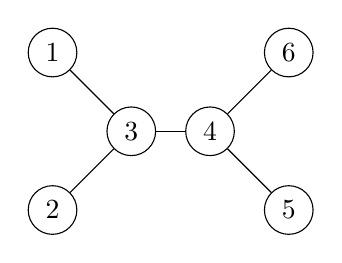
\begin{tikzpicture}
	\node[shape=circle,draw=black] (1) at (0,2) {1};
	\node[shape=circle,draw=black] (2) at (0,0) {2};
	\node[shape=circle,draw=black] (3) at (1,1) {3};
	\node[shape=circle,draw=black] (4) at (2,1) {4};
	\node[shape=circle,draw=black] (5) at (3,0) {5};
	\node[shape=circle,draw=black] (6) at (3,2) {6};
	
	\path [-] (1) edge node[left] {} (3);
	\path [-] (2) edge node[left] {} (3);
	\path [-] (3) edge node[left] {} (4);
	\path [-] (4) edge node[left] {} (5);
	\path [-] (4) edge node[left] {} (6);
\end{tikzpicture}

\section{Psudokod algorytmu}

\section{Dowód poprawności}

\section{Złożoność obliczeniowa}

\section{Format wejścia i wyjścia}

\newpage

\begin{thebibliography}{}

\end{thebibliography}

\end{document}